\documentclass[aspectratio=169]{beamer}

\usepackage{tikz}
\usetikzlibrary{decorations.pathmorphing}
\usetikzlibrary{decorations.pathreplacing}
\usetikzlibrary{calc,intersections}

\usepackage{pgfplots}
\usepackage{pgfplotstable}
\pgfplotsset{compat=1.18}
\usepgfplotslibrary{fillbetween}
\usepackage{csvsimple}
\usepackage{graphicx}
\usepackage{xcolor}

% LIGHTCONES
\newcommand{\lightconecurved}[5]{% x0=#1, t0=#2, length L=#3 % interior or exterior \pm
	\begin{scope}
		% 1. Inputs
		\pgfmathsetmacro{\xzero}{#1}
		\pgfmathsetmacro{\tzero}{#2}
		\pgfmathsetmacro{\raylen}{#3}
		\pgfmathsetmacro{\region}{#4}
		\pgfmathsetmacro{\rs}{#5}
		
		% 2. Slopes
		\pgfmathsetmacro{\sqrtterm}{sqrt(\rs/\xzero)}
		\pgfmathsetmacro{\den}{1 - \rs/\xzero}
		\pgfmathsetmacro{\mplus}{(\sqrtterm + 1)/(\den)}
		\pgfmathsetmacro{\mminus}{(\sqrtterm - 1)/(\den)}
		
		% 3. Normalization of length of light cone branches
		% Right branch (Positive x direction)
		\pgfmathsetmacro{\drR}{\raylen / sqrt((\mplus)^2 + 1)}
		\pgfmathsetmacro{\xfinr}{\xzero + \region*\drR}
		\pgfmathsetmacro{\tfinr}{\tzero + \region*\mplus * \drR}
		
		% Left branch (Negative x direction)
		\pgfmathsetmacro{\drL}{\raylen / sqrt((\mminus)^2 + 1)}
		\pgfmathsetmacro{\xfinl}{\xzero - \drL}
		\pgfmathsetmacro{\tfinl}{\tzero + \mminus * (-\drL)} % slope * negative change
		
		% 4. "Bake" values to avoid scope errors
		\edef\tempdraw{%
			\noexpand\draw[thick, red] (axis cs:\xzero,\tzero) -- (axis cs:\xfinr,\tfinr);
			\noexpand\draw[thick, red] (axis cs:\xzero,\tzero) -- (axis cs:\xfinl,\tfinl);
			\noexpand\fill[yellow, opacity=0.6] (axis cs:\xzero,\tzero) -- (axis cs:\xfinr,\tfinr) -- (axis cs:\xfinl,\tfinl) -- cycle;
		}
		\tempdraw
	\end{scope}
}

% Options
% 	[anonymous]	Provides output without author names, affiliations or acknowledgments to facilitate double-anonymous peer-review

\begin{document}

\title{Relativity through diagrams}
%\subtitle{A classroom-ready sequence of figures\\from spacetime diagrams to black holes}
\author{Mateo Paulišić}
\institute{Faculty of Physics, University of Rijeka}
\date{Extracted figures from\\"Diagrammatic approaches to teaching special and general relativity"}

\begin{frame}
	\titlepage
\end{frame}
	
\begin{frame}
	\centering
	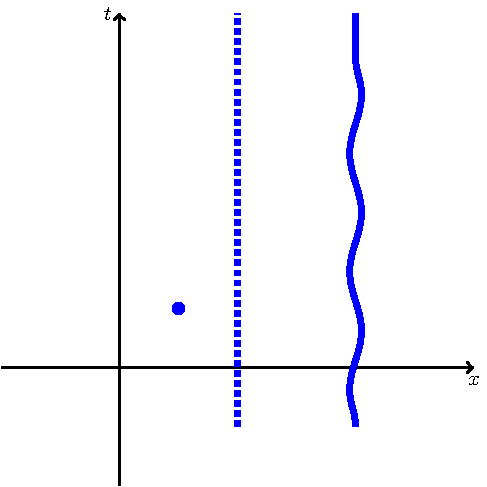
\includegraphics[page=1, width = 0.4\linewidth]{../figures/figures.pdf}
	
	\vspace{0.3em}
{\footnotesize A simple spacetime diagram with an emphasized single event, a series of events at a fixed position (which can be continued to a worldline of a stationary observer) and a worldline of a particle moving left and right.}
\end{frame}

\begin{frame}
	\centering
	\includegraphics[page=2, width = 0.4\linewidth]{../figures/figures.pdf}
	
\vspace{0.3em}
{\footnotesize A spacetime diagram with three slices of simultaneity (horizontal lines) and events marked as black dots. Each horizontal line represents events that are simultaneous from the perspective of the stationary observer.}
\end{frame}

\begin{frame}
	\centering
	\begin{minipage}{0.4\textwidth}
		\includegraphics[page=3, width = 1\linewidth]{../figures/figures.pdf}
	\end{minipage}
	\begin{minipage}{0.4\textwidth}
\includegraphics[page=4, width = 1\linewidth]{../figures/figures.pdf}
	\end{minipage}
	
\vspace{0.3em}
{\footnotesize The blue observer is moving to the right. The marked events represent ticking of a clock carried by each observer. Everyday experience tells us that stationary and moving clocks tick simultaneously, no matter who is observing.}
\end{frame}
\begin{frame}
	\centering
	\begin{minipage}
{0.4\textwidth}
		\includegraphics[page=5, width = 1\linewidth]{../figures/figures.pdf}
	\end{minipage}
	\begin{minipage}{0.4\textwidth}
		\includegraphics[page=6, width = 1\linewidth]{../figures/figures.pdf}
\end{minipage}

\vspace{0.3em}
{\footnotesize Spacetime diagrams with laboratory axes and the worldline of a light ray moving right. A light ray must cut the diagrams through the middle.}
\end{frame}

\begin{frame}
	\centering
	\begin{minipage}
		{0.4\textwidth}
		\includegraphics[page=7, width = 1\linewidth]{../figures/figures.pdf}
	\end{minipage}
	\begin{minipage}{0.4\textwidth}
		\includegraphics[page=8, width = 1\linewidth]{../figures/figures.pdf}
	\end{minipage}
	
	\vspace{0.3em}
{\footnotesize A spacetime diagram with a worldline of a light ray and a worldline of a moving observer, along with the tilted space axis of the moving observer. This is the crux of the pictorial argument for the relativity of simultaneity; the moving observer's space axis is tilted to ensure the that light ray bisects the angle between the time and space axes, thus preserving the invariance of the speed of light.}
\end{frame}

\begin{frame}
	\centering
	\includegraphics[page=9, width = 0.4\linewidth]{../figures/figures.pdf}
	
\vspace{0.3em}
{\footnotesize A spacetime diagram illustrating the relativity of simultaneity. The two black dots represent events that are simultaneous for the stationary observer (lying on the same horizontal line), but not for the moving observer (lying on different tilted lines), for whom the right event occurs earlier than the left one.}
\end{frame}

\begin{frame}
	\centering
	\includegraphics[page=10, width = 0.4\linewidth]{../figures/figures.pdf}
	
\vspace{0.3em}
{\footnotesize If both observers agreed on the time interval between ticks, this would contradict the relativity of simultaneity.}
\end{frame}
\begin{frame}
	\centering
	\begin{minipage}{0.4\textwidth}
		\includegraphics[page=11, width = 1\linewidth]{../figures/figures.pdf}
	\end{minipage}
	\begin{minipage}{0.4\textwidth}
		\includegraphics[page=12, width = 1\linewidth]{../figures/figures.pdf}
\end{minipage}

\vspace{0.3em}
{\footnotesize Left figure: readout of 1 second on a moving clock is simultaneous with more than 1 second on a stationary clock.\\Right figure: Readout of 1 second on a moving clock is simultaneous with less than 1 second on a stationary clock}
\end{frame}
\begin{frame}
	\centering
	\includegraphics[page=14, width = 0.35\linewidth]{../figures/figures.pdf}
	
\vspace{0.3em}
{\footnotesize No matter how the particle moves, its future is always confined within the light cone.}
\end{frame}


\begin{frame}
	\centering
	\includegraphics[page=15, width = 0.35\linewidth]{../figures/figures.pdf}
	
\vspace{0.3em}
{\footnotesize An array of freely falling particles. The light cones along their worldlines all have the same orientation.}
\end{frame}

\begin{frame}
	\centering
	\includegraphics[page=16, width = 0.4\linewidth]{../figures/figures.pdf}
	
\vspace{0.3em}
{\footnotesize Several particles in free-fall towards a central body (shaded)}
\end{frame}

\begin{frame}
	\centering
	\includegraphics[page=17, width = 0.4\linewidth]{../figures/figures.pdf}
	
\vspace{0.3em}
{\footnotesize Several particles in free-fall towards a central body (shaded) with light cones drawn at calculated locations. The light cones tilt as they approach the gravitating body.}
\end{frame}

\begin{frame}
	\centering
	\includegraphics[page=18, width = 0.4\linewidth]{../figures/figures.pdf}
	
\vspace{0.3em}
{\footnotesize An array of particles in free-fall towards a black hole. Once they cross the horizon (dashed line), the light cones tip over so much that their entire future is directed inward.}
\end{frame}






\end{document}


